\documentclass[12pt]{article}

\usepackage{amsmath, amssymb, amsfonts}
\usepackage{kotex}

\usepackage{geometry}
\usepackage{booktabs}
\usepackage{array}
\usepackage{multirow}
\usepackage{graphicx}
\usepackage{float}
\usepackage{indentfirst}
\usepackage{listings}
\usepackage{xcolor}

\newcommand{\x}{40pt}

\lstset{
    language=Python,
    basicstyle=\ttfamily\small,
    keywordstyle=\color{blue},
    commentstyle=\color{gray},
    stringstyle=\color{orange},
    breaklines=true,
    frame=single
}


\geometry{a4paper, margin=1in}

\title{Studies in Econometrics \\ Homework \#2}
\author{Park Jimin}
\date{2026-04-19}

\begin{document}

\maketitle

\section{Problem I}

We observe the profit of 100 firms in an industry. Let the sample be
\[
Y_1,\dots,Y_{100},
\]
where profit is measured in units of \$1,000.


\begin{figure}[H]
\centering
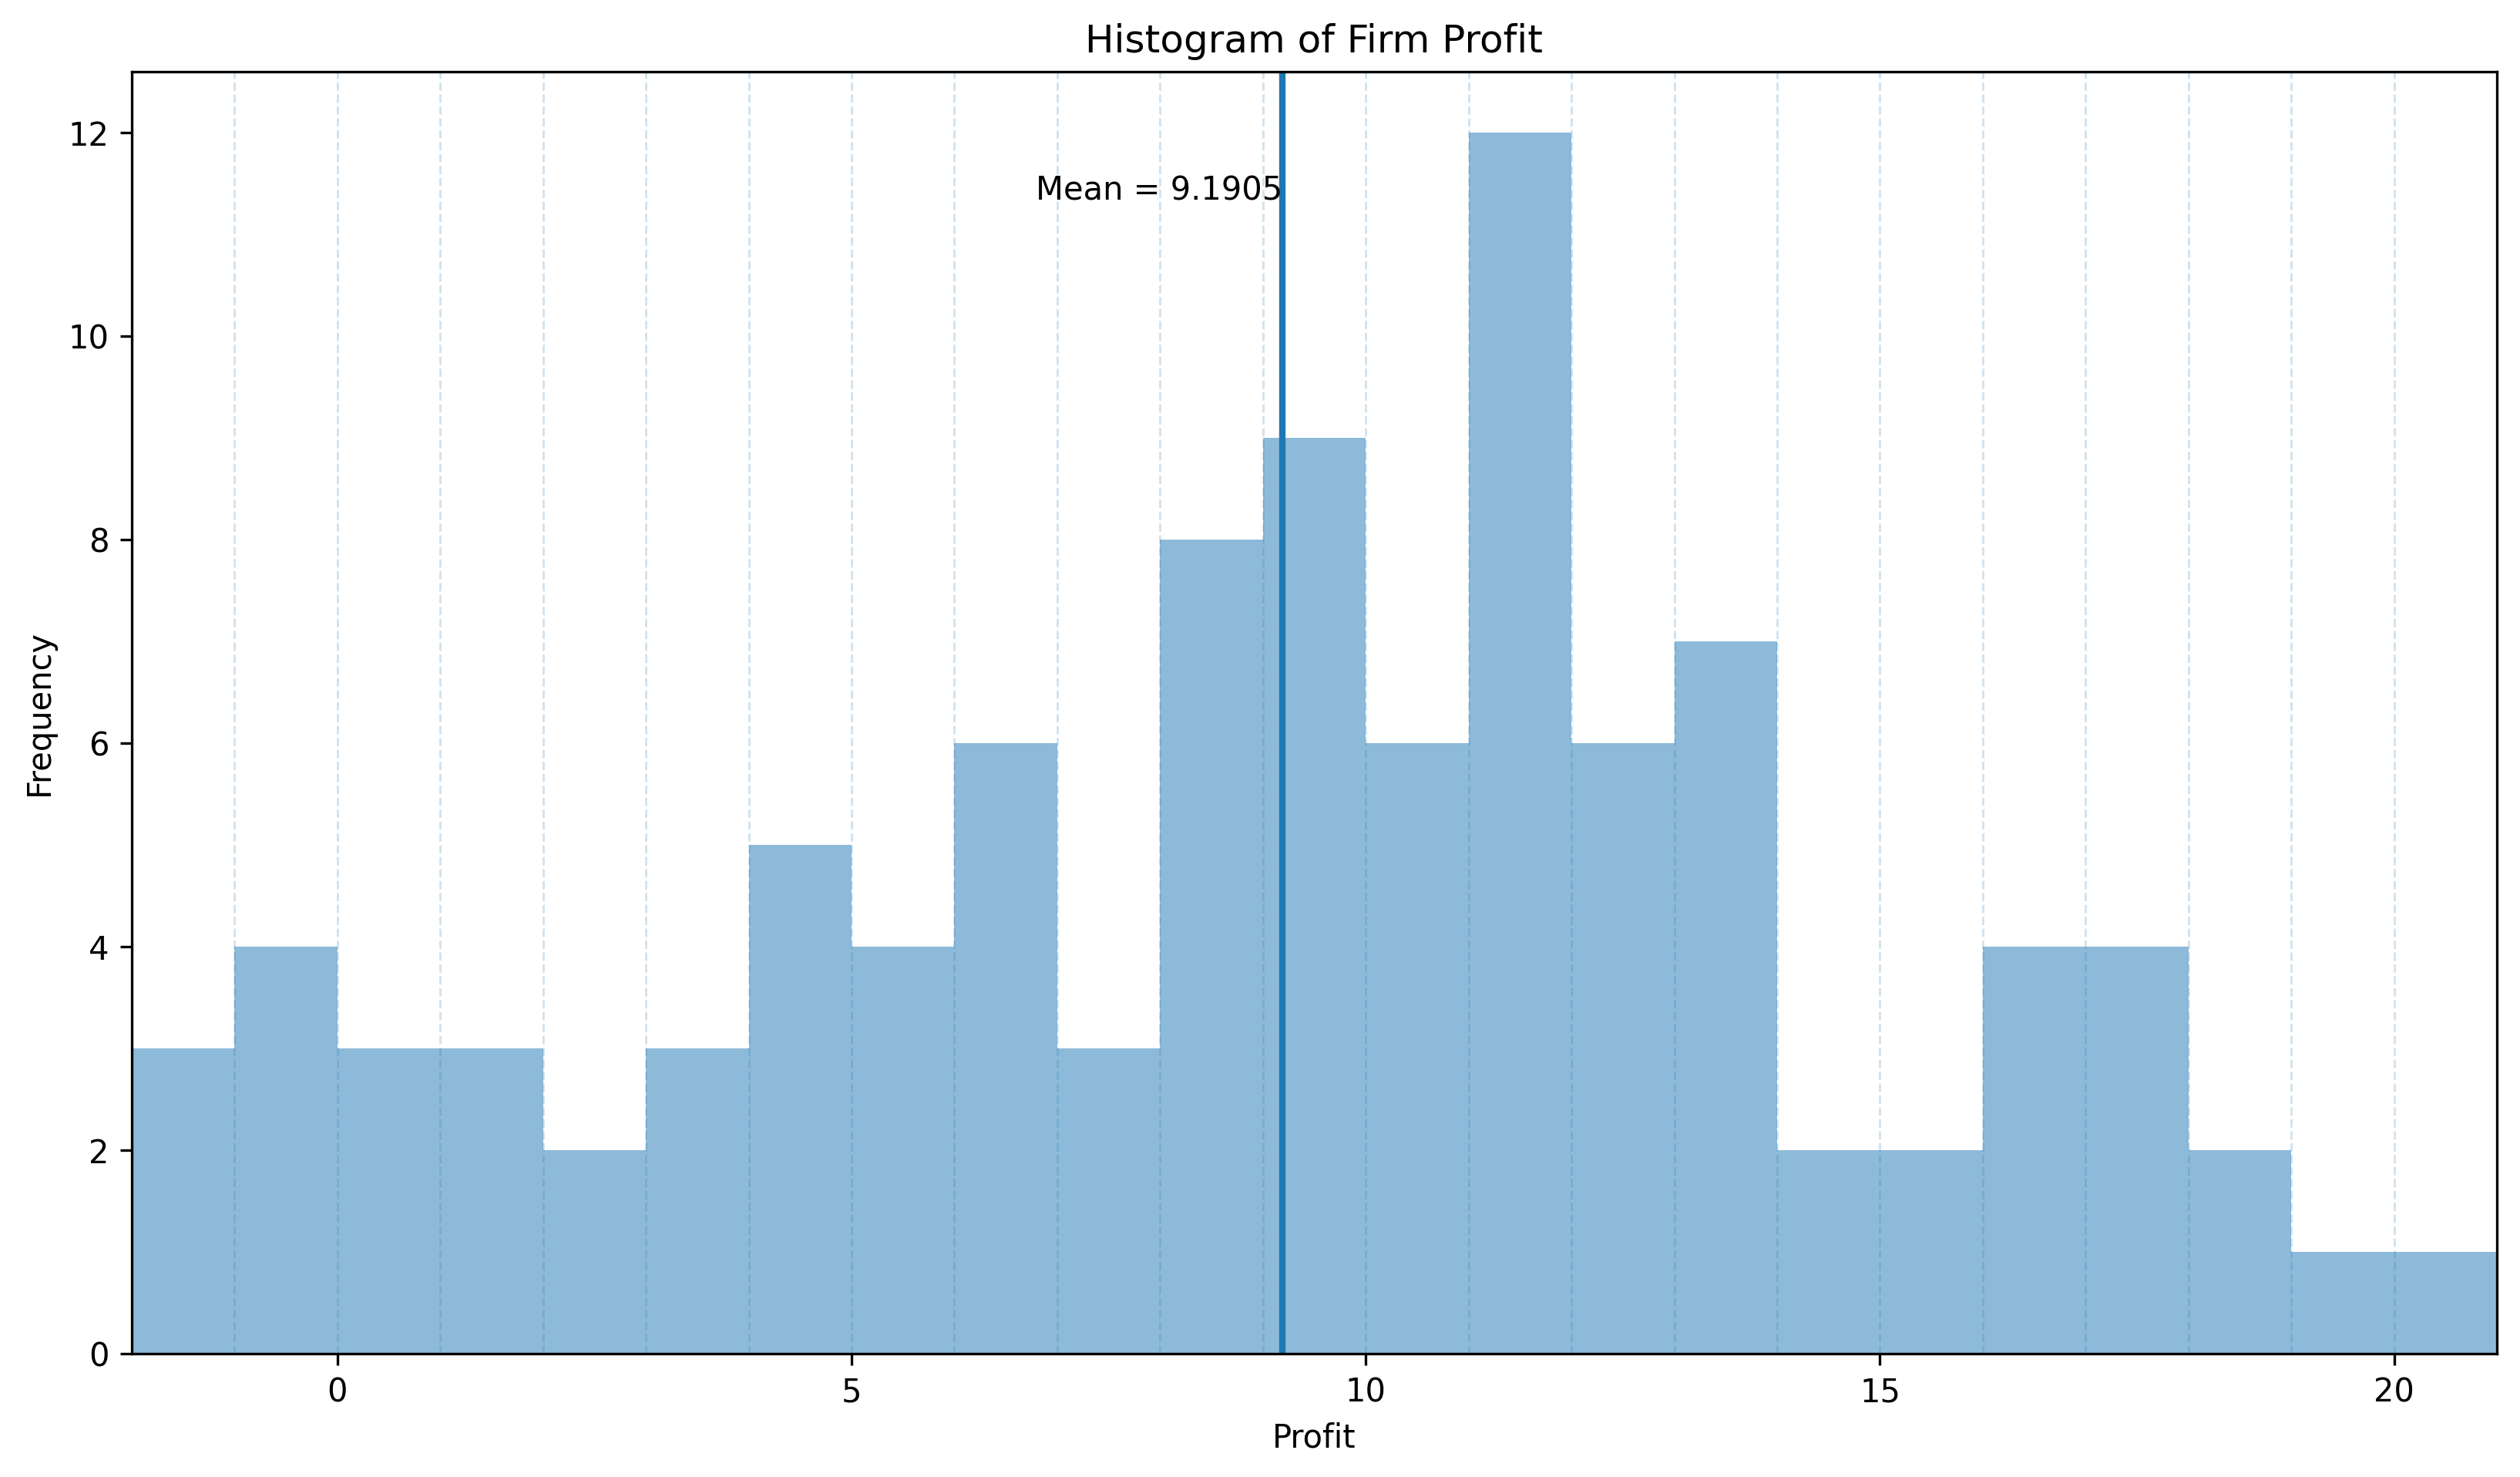
\includegraphics[width=\textwidth]{profit_plot.png}
\caption{Dot Plot of Firm Profit Distribution (Bin Width = 1) with Mean}
\end{figure}


\subsection{Mean Profit per Firm}

\subsubsection{Estimator and Its Properties}

Let \(\beta = E(Y_i)\) denote the population mean profit per firm.  
A natural estimator is \textbf{the 1st sample moment} of the random variable Y:
\[
\hat{\mu}_1 = \hat \beta = \frac{1}{100}\sum_{i=1}^{100} Y_i.
\]

Under random sampling, this estimator has the following properties:
\begin{itemize}
    \item \textbf{Unbiasedness:}
    \[
    E(\hat \beta) = \beta.
    \]
    \item \textbf{Variance:}
    \[
    \operatorname{Var}(\hat \beta) = \frac{\sigma^2}{100},
    \]
    where \(\sigma^2 = \operatorname{Var}(Y_i)\).
    \item \textbf{Consistency:} \(\hat \beta \xrightarrow{p} \beta\).
    \item \textbf{Asymptotic normality:}
    \[
    \sqrt{100}(\hat \beta-\beta)\xrightarrow{d}N(0,\sigma^2).
    \]
\end{itemize}

If profits are normally distributed, then \(\hat \beta\) is also the maximum likelihood estimator.

\subsubsection{Estimate of the Mean}

Using the sample data, the estimated mean profit per firm is
\[
\hat \beta = 9.190527.
\]

Since the unit is \$1{,}000, this corresponds to
\[
\$9{,}190.527.
\]
\subsection{Variance of Profit per Firm}

\subsubsection{Estimators and Their Properties}

Let \(\sigma^2 = \operatorname{Var}(Y_i)\) denote the population variance.

We consider two standard estimators.

\paragraph{Maximum likelihood estimator}
\[
\hat{\sigma}^2_{ML}
=
\frac{1}{100}\sum_{i=1}^{100}(Y_i-\hat{\beta})^2.
\]

Under the assumption of normality, this is the maximum likelihood estimator. It is biased in finite samples:
\[
E(\hat{\sigma}^2_{ML})=\frac{99}{100}\sigma^2,
\]
but it is consistent and asymptotically efficient.

\paragraph{Unbiased sample variance}
\[
\hat{\sigma}^2_{u}
=
\frac{1}{99}\sum_{i=1}^{100}(Y_i-\hat{\beta})^2.
\]

This estimator satisfies
\[
E(\hat{\sigma}^2_{u})=\sigma^2,
\]
and is therefore unbiased. It is also consistent.

\medskip

In summary, \(\hat{\sigma}^2_{ML}\) is derived from the likelihood function and is asymptotically efficient, while \(\hat{\sigma}^2_{u}\) corrects the finite-sample bias and provides an unbiased estimate of the population variance.

\subsubsection{Estimate of the Variance}

Using the sample data, we obtain
\[
\hat{\sigma}^2_{ML}=28.532358,
\qquad
\hat{\sigma}^2_{u}=28.820563.
\]

Since the sample size is finite, we report the unbiased estimator \(\hat{\sigma}^2_{u}\) as the estimate of the variance. Therefore, the variance of profit per firm is estimated to be approximately 28.82.


\subsection{Test of the Hypothesis that Mean Profit Equals \$10,000}

The analyst claims that the mean profit per firm is \$10,000. Since the data are measured in units of \$1,000, this corresponds to the hypothesis
\[
H_0:\beta_0 = 10,
\qquad
H_1:\beta_0 \neq 10.
\]

\subsubsection{Likelihood Ratio Test: Definition and Intuition}

The likelihood ratio (LR) test compares the maximized likelihood under the unrestricted parameter space \(\Omega\) and the restricted space \(\Omega_0\). Formally,
\[
\lambda
=
\frac{l^*(\Omega)}{l^*(\Omega_0)}.
\]

If the restriction imposed by \(H_0\) significantly increases the likelihood ratio, the null hypothesis is rejected.

\subsubsection{Implementation of the Likelihood Ratio Test}

Assume
\[
Y_i \overset{i.i.d.}{\sim} N(\beta,\sigma^2).
\]

Under the unrestricted model, the estimators are
\[
\hat{\beta} = \frac{1}{100}\sum_{i=1}^{100} Y_i,
\qquad
\hat{\sigma}_{ML}^2
=
\frac{1}{100}\sum_{i=1}^{100}(Y_i-\hat{\beta})^2.
\]

Under the null hypothesis \(H_0:\beta_0 = 10\), the restricted variance estimator is
\[
\hat{\sigma}_0^2
=
\frac{1}{100}\sum_{i=1}^{100}(Y_i-10)^2.
\]

The likelihood ratio can be written as
\[
\lambda
=
\frac{l^*(\Omega)}{l^*(\Omega_0)}
=
\left(
\frac{\hat{\sigma}_0^2}{\hat{\sigma}_{ML}^2}
\right)^{T/2}.
\]

To obtain a statistic with a known finite-sample distribution, consider the monotonic transformation
\[
\lambda^*
=
(T-1)\left(\lambda^{2/T}-1\right).
\]

It can be shown that this simplifies to
\[
\lambda^*
=
\frac{(\hat{\beta}-\beta_0)^2}{\hat{\sigma}_u^2/T},
\]
where
\[
\hat{\sigma}_u^2
=
\frac{1}{T-1}\sum_{i=1}^{100}(Y_i-\hat{\beta})^2
\]
is the unbiased variance estimator.

Under \(H_0\),
\[
\lambda^* \sim F(1, T-1).
\]

Taking the square root yields
\[
t^*
=
\sqrt{\lambda^*}
=
\frac{|\hat{\beta}-\beta_0|}{\sqrt{\hat{\sigma}_u^2/T}},
\]
and hence
\[
\frac{\hat{\beta}-\beta_0}{\sqrt{\hat{\sigma}_u^2/T}}
\sim t(T-1).
\]

Thus, the LR test is equivalent to the standard \(t\)-test.

\paragraph{Numerical implementation}

Using the data,
\[
\hat{\beta} = 9.190527,
\qquad
\hat{\sigma}_{ML}^2 = 28.532358,
\qquad
\hat{\sigma}_0^2 = 29.187604,
\qquad
\hat{\sigma}_u^2 = 28.820563.
\]

The test statistic is
\[
t
=
\frac{\hat{\beta}-10}{\sqrt{\hat{\sigma}_u^2/100}}
=
\frac{9.190527-10}{\sqrt{28.820563}/10}
=
-1.507826.
\]

Thus,
\[
\lambda^* = t^2 = 2.273538.
\]

Under \(H_0\),
\[
t \sim t(99),
\qquad
\lambda^* \sim F(1,99).
\]

The two-sided \(p\)-value is
\[
p = 0.134784.
\]

Therefore, at the 5\% significance level, we fail to reject \(H_0\).

\paragraph{Asymptotic LR version}

Alternatively, consider the asymptotic LR statistic
\[
LR
=
2\ln\left(
\frac{l^*(\Omega)}{l^*(\Omega_0)}
\right)
=
T\ln\left(\frac{\hat{\sigma}_0^2}{\hat{\sigma}^2}\right).
\]

Using the data,
\[
LR
=
100\ln\left(\frac{29.187604}{28.532358}\right)
=
2.270531.
\]

Under \(H_0\),
\[
LR \xrightarrow{d} \chi^2(1).
\]

The corresponding \(p\)-value is
\[
p = 0.131855.
\]

Since this exceeds 0.05, we again fail to reject \(H_0\).

\subsubsection{Assumptions and Interpretation}

The finite-sample results rely on the assumption that
\[
Y_i \overset{i.i.d.}{\sim} N(\beta,\sigma^2).
\]

The asymptotic LR test requires only random sampling and regularity conditions.

Both approaches lead to the same conclusion: there is insufficient evidence to reject the hypothesis that the mean profit per firm is \$10,000. Although the sample mean is below this value, the difference is not statistically significant.
\section{Problem II}

Let \((Y_1,\dots,Y_T)\) be a random sample from a normal distribution:
\[
Y_t \sim N(\beta,\sigma^2),
\qquad t=1,\dots,T.
\]

\subsection{Log-Likelihood Function and Maximum Likelihood Estimators}

The density of \(Y_t\) is
\[
f(y_t\mid \beta,\sigma^2)
=
\frac{1}{\sqrt{2\pi\sigma^2}}
\exp\left(
-\frac{(y_t- \beta)^2}{2\sigma^2}
\right).
\]

Hence, the likelihood function of the sample is
\[
l(\beta,\sigma^2)
=
\prod_{t=1}^T
\frac{1}{\sqrt{2\pi\sigma^2}}
\exp\left(
-\frac{(y_t-\beta)^2}{2\sigma^2}
\right),
\]
which can be written as
\[
l(\beta,\sigma^2)
=
(2\pi\sigma^2)^{-T/2}
\exp\left(
-\frac{1}{2\sigma^2}\sum_{t=1}^T (y_t-\beta)^2
\right).
\]

Therefore, the log-likelihood function is
\[
L(\beta,\sigma^2)
=
-\frac{T}{2}\ln(2\pi)
-\frac{T}{2}\ln(\sigma^2)
-\frac{1}{2\sigma^2}\sum_{t=1}^T (y_t-\beta)^2.
\]

To find the MLE, differentiate with respect to \(\beta\):
\[
\frac{\partial L}{\partial \beta}
=
\frac{1}{\sigma^2}\sum_{t=1}^T (y_t-\beta).
\]
Setting this equal to zero gives
\[
\sum_{t=1}^T(y_t-\beta)=0
\quad \Rightarrow \quad
\hat \beta=\frac{1}{T}\sum_{t=1}^T Y_t.
\]

Next, differentiate with respect to \(\sigma^2\):
\[
\frac{\partial L}{\partial \sigma^2}
=
-\frac{T}{2\sigma^2}
+\frac{1}{2\sigma^4}\sum_{t=1}^T (y_t-\beta)^2.
\]
Setting this equal to zero yields
\[
\hat{\sigma}^2
=
\frac{1}{T}\sum_{t=1}^T (Y_t-{\hat \beta})^2.
\]

Thus, the maximum likelihood estimators are
\[
\boxed{
\hat{\beta}=\frac{1}{T}\sum_{t=1}^T Y_t
}
\]
and
\[
\boxed{
\hat{\sigma}^2=\frac{1}{T}\sum_{t=1}^T (Y_t-\hat \beta)^2
}.
\]

\paragraph{Properties}

The estimator \({\hat \beta}\) is unbiased:
\[
E({\hat \beta})=\beta,
\qquad
\operatorname{Var}({\hat \beta})=\frac{\sigma^2}{T}.
\]
Hence, \(\hat{\hat \beta}\) is consistent and asymptotically normal.

The estimator \(\hat{\sigma}^2\) is the MLE, but it is biased:
\[
E(\hat{\sigma}^2)=\frac{T-1}{T}\sigma^2.
\]
However, it is consistent.

\subsection{Information Matrix and Asymptotic Distribution}

Let
\[
\theta=
\begin{pmatrix}
\beta\\
\sigma^2
\end{pmatrix}.
\]

The second derivatives of the log-likelihood are
\[
\frac{\partial^2 \ell}{\partial \beta^2}
=
-\frac{T}{\sigma^2},
\]
\[
\frac{\partial^2 \ell}{\partial \beta \,\partial \sigma^2}
=
-\frac{1}{\sigma^4}\sum_{t=1}^T(Y_t-\beta),
\]
and
\[
\frac{\partial^2 \ell}{\partial (\sigma^2)^2}
=
\frac{T}{2\sigma^4}
-
\frac{1}{\sigma^6}\sum_{t=1}^T(Y_t-\beta)^2.
\]

Taking expectations,
\[
E\left[\frac{\partial^2 \ell}{\partial \beta \,\partial \sigma^2}\right]=0,
\]
and
\[
E\left[\frac{\partial^2 \ell}{\partial (\sigma^2)^2}\right]
=
-\frac{T}{2\sigma^4}.
\]

Therefore, the information matrix is
\[
I(\theta)
=
-E\left[
\frac{\partial^2 \ell(\theta)}{\partial \theta \partial \theta'}
\right]
=
\begin{pmatrix}
T/\sigma^2 & 0\\
0 & T/(2\sigma^4)
\end{pmatrix}.
\]

Its inverse is
\[
I(\theta)^{-1}
=
\begin{pmatrix}
\sigma^2/T & 0\\
0 & 2\sigma^4/T
\end{pmatrix}.
\]

Hence, the MLE is asymptotically distributed as
\[
\sqrt{T}
\begin{pmatrix}
\hat{\beta}-\beta\\
\hat{\sigma}^2-\sigma^2
\end{pmatrix}
\xrightarrow{d}
N\left(
\begin{pmatrix}
0\\
0
\end{pmatrix},
\begin{pmatrix}
\sigma^2 & 0\\
0 & 2\sigma^4
\end{pmatrix}
\right).
\]

Equivalently, for large \(T\),
\[
\hat{\beta}\approx N\left(\beta,\frac{\sigma^2}{T}\right),
\qquad
\hat{\sigma}^2\approx N\left(\sigma^2,\frac{2\sigma^4}{T}\right).
\]


\newpage

\appendix
\section*{Appendix: Python Code}

\begin{lstlisting}
import pandas as pd
import numpy as np
from scipy import stats

# =========================
# 1. Load data
# =========================
file_path = "/home/wlals788/workspace/python/1_src/assignments/econometrics_2/HW2 data.csv"
df = pd.read_csv(file_path)

print("Columns in dataset:", df.columns.tolist())
print(df.head())

# -------------------------
# Select variable
# -------------------------
y = df["profit"]

y = y.to_numpy()
n = len(y)


# =========================
# 2. Mean and variance estimation
# =========================
y_bar = np.mean(y)

# MLE variance (denominator n)
sigma2_ml = np.mean((y - y_bar) ** 2)

# Unbiased variance (denominator n-1)
s2_unbiased = np.var(y, ddof=1)

print("\n[1] Mean Estimation")
print(f"Sample mean = {y_bar:.6f}")

print("\n[2] Variance Estimation")
print(f"MLE variance = {sigma2_ml:.6f}")
print(f"Unbiased variance = {s2_unbiased:.6f}")

# =========================
# 3. Hypothesis test: H0: mu = 10
# =========================
mu0 = 10.0

# Small-sample t-test
s = np.sqrt(s2_unbiased)
t_stat = (y_bar - mu0) / (s / np.sqrt(n))
p_value_t = 2 * (1 - stats.t.cdf(abs(t_stat), df=n - 1))

# Finite-sample LR equivalent statistic
F_stat = t_stat ** 2
p_value_F = 1 - stats.f.cdf(F_stat, 1, n - 1)

# Restricted variance under H0
sigma2_0 = np.mean((y - mu0) ** 2)

# Asymptotic LR statistic
LR = n * np.log(sigma2_0 / sigma2_ml)
p_value_LR = 1 - stats.chi2.cdf(LR, df=1)

print("\n[3] Hypothesis Test: H0: mu = 10 vs H1: mu != 10")
print(f"Restricted variance under H0 = {sigma2_0:.6f}")

print("\nSmall-sample version (t-test equivalent)")
print(f"t statistic = {t_stat:.6f}")
print(f"Two-sided p-value (t-test) = {p_value_t:.6f}")
print(f"F statistic (t^2) = {F_stat:.6f}")
print(f"p-value (F distribution) = {p_value_F:.6f}")

print("\nAsymptotic Likelihood Ratio Test")
print(f"LR statistic = {LR:.6f}")
print(f"p-value (chi-square(1)) = {p_value_LR:.6f}")

# =========================
# 4. Decision at 5% level
# =========================
alpha = 0.05

print("\n[4] Decision at 5% significance level")

if p_value_t < alpha:
    print("Small-sample test: Reject H0")
else:
    print("Small-sample test: Fail to reject H0")

if p_value_LR < alpha:
    print("Asymptotic LR test: Reject H0")
else:
    print("Asymptotic LR test: Fail to reject H0")
\end{lstlisting}

\end{document}